% answers.tex —— 2013 年·辽宁卷·文科 · 参考答案与详细解析片段
% 由 tools/generate_projects.py 依来源总账自 2013/2013_数学真题_辽宁文_试题.md + 2013/2013_数学真题_辽宁文_解析正文.md + 2013/2013_数学真题_辽宁文_答案要点.md 生成，勿手改（改源 MD 后重跑）

\begin{answer}
\gksolhead{1}{}

\textbf{题目}：

已知集合 $A=\{0,1,2,3,4\}$，$B=\{x\mid |x|<2\}$，则 $A\cap B=$\mbox{（　　）}

（A）$\{0\}$；（B）$\{0,1\}$；（C）$\{0,2\}$；（D）$\{0,1,2\}$。

\Needspace{4\baselineskip}
\textbf{解析}
\Needspace{5\baselineskip}
由 $|x|<2$ 得 $-2<x<2$，所以
\nopagebreak[4]
\[B=\{x\mid -2<x<2\}.\]
\Needspace{5\baselineskip}
集合 $A$ 中的元素只有 $0$，$1$ 满足该条件（$2$，$3$，$4$ 都不满足），故
\nopagebreak[4]
\[A\cap B=\{0,1\}.\]
选 B。

\gkanswer{答案：B。}

\end{answer}
\begin{answer}
\gksolhead{2}{}

\textbf{题目}：

复数 $z=\dfrac{1}{\mathrm i-1}$ 的模为\mbox{（　　）}

（A）$\dfrac12$；（B）$\dfrac{\sqrt2}2$；（C）$\sqrt2$；（D）$2$。

\Needspace{4\baselineskip}
\textbf{解析}
\Needspace{5\baselineskip}
由复数模的性质，
\nopagebreak[4]
\[|z|=\left|\frac{1}{\mathrm i-1}\right|=\frac{1}{|\mathrm i-1|}=\frac{1}{\sqrt{1^2+(-1)^2}}=\frac1{\sqrt2}=\frac{\sqrt2}2.\]
选 B。

\gkanswer{答案：B。}

\end{answer}
\begin{answer}
\gksolhead{3}{}

\textbf{题目}：

已知点 $A(1,3)$，$B(4,-1)$，则与向量 $\overrightarrow{AB}$ 同方向的单位向量为\mbox{（　　）}

（A）$\left(\dfrac35,-\dfrac45\right)$；（B）$\left(\dfrac45,-\dfrac35\right)$；（C）$\left(-\dfrac35,\dfrac45\right)$；（D）$\left(-\dfrac45,\dfrac35\right)$。

\Needspace{4\baselineskip}
\textbf{解析}
\nopagebreak[4]
\[\overrightarrow{AB}=(4-1,\,-1-3)=(3,-4),\]
\Needspace{5\baselineskip}
其模为
\nopagebreak[4]
\[|\overrightarrow{AB}|=\sqrt{3^2+(-4)^2}=5.\]
\Needspace{5\baselineskip}
与 $\overrightarrow{AB}$ 同方向的单位向量为
\nopagebreak[4]
\[\frac{\overrightarrow{AB}}{|\overrightarrow{AB}|}=\left(\frac35,-\frac45\right).\]
选 A。

\gkanswer{答案：A。}

\end{answer}
\begin{answer}
\gksolhead{4}{}

\textbf{题目}：

下面是关于公差 $d>0$ 的等差数列 $\{a_n\}$ 的四个命题：

$p_1$：数列 $\{a_n\}$ 是递增数列；

$p_2$：数列 $\{na_n\}$ 是递增数列；

$p_3$：数列 $\left\{\dfrac{a_n}{n}\right\}$ 是递增数列；

$p_4$：数列 $\{a_n+3nd\}$ 是递增数列。

其中的真命题为\mbox{（　　）}

（A）$p_1$，$p_2$；（B）$p_3$，$p_4$；（C）$p_2$，$p_3$；（D）$p_1$，$p_4$。

\Needspace{4\baselineskip}
\textbf{解析}
设 $a_n=a_1+(n-1)d$，其中 $d>0$。

\begin{itemize}
\item $p_1$：$a_{n+1}-a_n=d>0$，故 $\{a_n\}$ 递增，真命题；
\item $p_2$：$(n+1)a_{n+1}-na_n=a_1+2nd$，当 $a_1$ 充分小（如 $a_1=-100$，$n=1$）时为负，故 $\{na_n\}$ 不一定是递增数列，假命题；
\item $p_3$：$\dfrac{a_n}{n}=d+\dfrac{a_1-d}{n}$，当 $a_1>d$ 时随 $n$ 增大而减小，故不一定是递增数列，假命题；
\item $p_4$：$(a_{n+1}+3(n+1)d)-(a_n+3nd)=d+3d=4d>0$，故 $\{a_n+3nd\}$ 递增，真命题。
\end{itemize}

真命题为 $p_1$，$p_4$。选 D。

\gkanswer{答案：D。}

\end{answer}
\begin{answer}
\gksolhead{5}{}

\textbf{题目}：

某班的全体学生参加英语测试，成绩的频率分布直方图如图，数据的分组依次为：$[20,40)$，$[40,60)$，$[60,80)$，$[80,100]$。若低于 $60$ 分的人数是 $15$，则该班的学生人数是\mbox{（　　）}
\nopagebreak[4]
\begin{center}% 2013 辽宁卷文科第 5 题：成绩频率分布直方图。
\begin{tikzpicture}[font=\footnotesize, >=Stealth, line width=0.5pt,
  x=1.15cm, y=160cm]
  % 坐标轴：横轴以 20 分为一个单位
  \draw[->] (0,0) -- (5.75,0) node[right, yshift=-2pt] {成绩/分};
  \draw[->] (0,0) -- (0,0.0238);
  \node at (0,0.0295) {$\dfrac{\text{频率}}{\text{组距}}$};
  % 横轴刻度
  \foreach \x/\lab in {0/0,1/20,2/40,3/60,4/80,5/100}
    \draw (\x,0) -- (\x,-0.0006) node[below] {$\lab$};
  % 纵轴刻度与虚线
  \foreach \y/\lab in {0.005/0.005,0.010/0.010,0.015/0.015,0.020/0.020} {
    \draw (0,\y) -- (-0.08,\y) node[left] {$\lab$};
    \draw[dashed] (0,\y) -- (5.05,\y);
  }
  % 四个矩形：高度依次为 0.005、0.010、0.020、0.015
  \foreach \i/\h in {1/0.005,2/0.010,3/0.020,4/0.015} {
    \draw[fill=white] (\i-1,0) rectangle (\i,\h);
  }
\end{tikzpicture}
\end{center}
\nopagebreak[4]
（A）$45$；（B）$50$；（C）$55$；（D）$60$。

\Needspace{4\baselineskip}
\textbf{解析}
\Needspace{5\baselineskip}
各组的频率为“组距 $\times$ 频率/组距”，组距均为 $20$。低于 $60$ 分的两组为 $[20,40)$ 与 $[40,60)$，其频率之和为
\nopagebreak[4]
\[(0.005+0.010)\times20=0.30.\]
\Needspace{5\baselineskip}
设该班学生人数为 $n$，则
\nopagebreak[4]
\[0.30n=15\implies n=50.\]
选 B。

\gkanswer{答案：B。}

\end{answer}
\begin{answer}
\gksolhead{6}{}

\textbf{题目}：

在 $\triangle ABC$ 中，内角 $A$，$B$，$C$ 所对的边分别为 $a$，$b$，$c$，若 $a\sin B\cos C+c\sin B\cos A=\dfrac12b$，且 $a>b$，则 $\angle B=$\mbox{（　　）}

（A）$\dfrac\pi6$；（B）$\dfrac\pi3$；（C）$\dfrac{2\pi}3$；（D）$\dfrac{5\pi}6$。

\Needspace{4\baselineskip}
\textbf{解析}
\Needspace{5\baselineskip}
由正弦定理 $a=2R\sin A$，$b=2R\sin B$，$c=2R\sin C$，代入已知式并除以 $2R\sin B$（$\sin B\neq0$）得
\nopagebreak[4]
\[\sin A\cos C+\cos A\sin C=\frac12.\]
\Needspace{5\baselineskip}
左边即 $\sin(A+C)=\sin(\pi-B)=\sin B$，故
\nopagebreak[4]
\[\sin B=\frac12.\]
\Needspace{5\baselineskip}
所以 $B=\dfrac\pi6$ 或 $B=\dfrac{5\pi}6$。若 $B=\dfrac{5\pi}6$，则 $A<\dfrac\pi6<B$，从而 $a<b$，与 $a>b$ 矛盾。故
\nopagebreak[4]
\[B=\frac\pi6.\]
选 A。

\gkanswer{答案：A。}

\end{answer}
\begin{answer}
\gksolhead{7}{}

\textbf{题目}：

已知函数 $f(x)=\ln\left(\sqrt{1+9x^2}-3x\right)+1$，则 $f(\lg 2)+f\left(\lg\dfrac12\right)=$\mbox{（　　）}

（A）$-1$；（B）$0$；（C）$1$；（D）$2$。

\Needspace{4\baselineskip}
\textbf{解析}
\Needspace{5\baselineskip}
记 $u(x)=\sqrt{1+9x^2}-3x$，则 $u(x)>0$，且
\nopagebreak[4]
\[u(x)u(-x)=\left(\sqrt{1+9x^2}\right)^2-(3x)^2=1+9x^2-9x^2=1.\]
\Needspace{5\baselineskip}
于是
\nopagebreak[4]
\[f(x)+f(-x)=\ln u(x)+1+\ln u(-x)+1=\ln 1+2=2.\]
\Needspace{5\baselineskip}
取 $x=\lg2$，则 $-x=\lg\dfrac12$，故
\nopagebreak[4]
\[f(\lg2)+f\left(\lg\frac12\right)=2.\]
选 D。

\gkanswer{答案：D。}

\end{answer}
\begin{answer}
\gksolhead{8}{}

\textbf{题目}：

执行如图所示的程序框图，若输入 $n=8$，则输出 $S=$\mbox{（　　）}
\nopagebreak[4]
\begin{center}% 2013 辽宁卷文科第 8 题：程序框图。
\begin{tikzpicture}[font=\footnotesize, >=Stealth, line width=0.45pt,
  node distance=5mm,
  term/.style={draw, rounded corners=6pt, minimum height=1.8em, inner xsep=9pt},
  io/.style={draw, trapezium, trapezium left angle=70, trapezium right angle=110,
             minimum height=1.8em, inner xsep=6pt},
  box/.style={draw, minimum height=1.9em, inner xsep=6pt},
  dec/.style={draw, diamond, aspect=2.2, inner sep=1pt}]
  \node[term] (start) {开始};
  \node[io, below=5mm of start] (input) {输入 $n$};
  \node[box, below=5mm of input] (init) {$S=0$，$i=2$};
  \node[dec, below=6mm of init] (cond) {$i\leqslant n$};
  \node[box, below=7mm of cond] (acc) {$S=S+\dfrac{1}{i^2-1}$};
  \node[box, below=5mm of acc] (inc) {$i=i+2$};
  \node[io, right=15mm of cond] (output) {输出 $S$};
  \node[term, below=6mm of output] (end) {结束};
  \draw[->] (start) -- (input);
  \draw[->] (input) -- (init);
  \draw[->] (init) -- (cond);
  \draw[->] (cond) -- node[right] {是} (acc);
  \draw[->] (acc) -- (inc);
  \draw[->] (cond) -- node[above] {否} (output);
  \draw[->] (output) -- (end);
  % 循环支路：从 i=i+2 左侧引出，向上回到判断框入口
  \draw[->] (inc.west) -- ++(-1.45,0) |- (cond.west);
\end{tikzpicture}
\end{center}
\nopagebreak[4]
（A）$\dfrac49$；（B）$\dfrac67$；（C）$\dfrac89$；（D）$\dfrac{10}{11}$。

\Needspace{4\baselineskip}
\textbf{解析}
\Needspace{5\baselineskip}
框图执行的循环体为
\nopagebreak[4]
\[S=S+\frac1{i^2-1},\qquad i=i+2,\]
\Needspace{5\baselineskip}
初值 $S=0$，$i=2$，当 $i\leqslant8$ 时依次取 $i=2,4,6,8$。由
\nopagebreak[4]
\[\frac1{i^2-1}=\frac1{(i-1)(i+1)}=\frac12\left(\frac1{i-1}-\frac1{i+1}\right),\]
\Needspace{5\baselineskip}
得
\nopagebreak[4]
\[S=\frac12\left[\left(1-\frac13\right)+\left(\frac13-\frac15\right)+\left(\frac15-\frac17\right)+\left(\frac17-\frac19\right)\right]
=\frac12\left(1-\frac19\right)=\frac49.\]
选 A。

\gkanswer{答案：A。}

\end{answer}
\begin{answer}
\gksolhead{9}{}

\textbf{题目}：

已知点 $O(0,0)$，$A(0,b)$，$B(a,a^3)$。若 $\triangle OAB$ 为直角三角形，则必有\mbox{（　　）}

（A）$b=a^3$；（B）$b=a^3+\dfrac1a$；（C）$(b-a^3)\left(b-a^3-\dfrac1a\right)=0$；（D）$\left|b-a^3\right|+\left|b-a^3-\dfrac1a\right|=0$。

\Needspace{4\baselineskip}
\textbf{解析}
\nopagebreak[4]
\[\overrightarrow{OA}=(0,b),\quad \overrightarrow{OB}=(a,a^3),\quad \overrightarrow{AB}=(a,a^3-b).\]
分别讨论直角顶点（$a\neq0$，$b\neq0$，否则三角形退化）：

\begin{itemize}
\item 若直角在 $O$：$\overrightarrow{OA}\cdot\overrightarrow{OB}=ba^3=0$，得 $b=0$，退化，舍去；
\item 若直角在 $A$：$\overrightarrow{AO}\cdot\overrightarrow{AB}=(0,-b)\cdot(a,a^3-b)=-b(a^3-b)=0$，得 $b=a^3$；
\item 若直角在 $B$：$\overrightarrow{BA}\cdot\overrightarrow{BO}=(-a,b-a^3)\cdot(-a,-a^3)=a^2-a^3(b-a^3)=0$，即 $b-a^3=\dfrac1a$。
\end{itemize}

\Needspace{5\baselineskip}
故必有
\nopagebreak[4]
\[(b-a^3)\left(b-a^3-\frac1a\right)=0.\]
选 C。

\gkanswer{答案：C。}

\end{answer}
\begin{answer}
\gksolhead{10}{}

\textbf{题目}：

已知直三棱柱 $ABC-A_1B_1C_1$ 的 $6$ 个顶点都在球 $O$ 的球面上。若 $AB=3$，$AC=4$，$AB\perp AC$，$AA_1=12$，则球 $O$ 的半径为\mbox{（　　）}

（A）$\dfrac{3\sqrt{17}}2$；（B）$2\sqrt{10}$；（C）$\dfrac{13}2$；（D）$3\sqrt{10}$。

\Needspace{4\baselineskip}
\textbf{解析}
\Needspace{5\baselineskip}
直三棱柱的外接球球心是上下底面外心连线的中点。底面 $\triangle ABC$ 中 $AB\perp AC$，故 $BC$ 为底面外接圆直径，
\nopagebreak[4]
\[BC=\sqrt{3^2+4^2}=5,\]
\Needspace{5\baselineskip}
底面外接圆半径 $r=\dfrac52$。球心到底面的距离为 $\dfrac{AA_1}2=6$，故球半径
\nopagebreak[4]
\[R=\sqrt{r^2+6^2}=\sqrt{\frac{25}4+36}=\sqrt{\frac{169}4}=\frac{13}2.\]
选 C。

\gkanswer{答案：C。}

\end{answer}
\begin{answer}
\gksolhead{11}{}

\textbf{题目}：

已知椭圆 $C:\dfrac{x^2}{a^2}+\dfrac{y^2}{b^2}=1\ (a>b>0)$ 的左焦点为 $F$，$C$ 与过原点的直线相交于 $A$，$B$ 两点，连接 $AF$，$BF$。若 $|AB|=10$，$|BF|=8$，$\cos\angle ABF=\dfrac45$，则 $C$ 的离心率为\mbox{（　　）}

（A）$\dfrac35$；（B）$\dfrac57$；（C）$\dfrac45$；（D）$\dfrac67$。

\Needspace{4\baselineskip}
\textbf{解析}
\Needspace{5\baselineskip}
在 $\triangle ABF$ 中，
\nopagebreak[4]
\[|AF|^2=|AB|^2+|BF|^2-2|AB|\cdot|BF|\cos\angle ABF
=100+64-2\times10\times8\times\frac45=36,\]
故 $|AF|=6$。于是 $|AF|^2+|BF|^2=36+64=100=|AB|^2$，所以 $\angle AFB=90^\circ$。

\Needspace{5\baselineskip}
设椭圆的右焦点为 $F'$。由 $A$，$B$ 关于原点 $O$ 对称，$F$，$F'$ 也关于 $O$ 对称，故四边形 $AFBF'$ 是平行四边形；又 $\angle AFB=90^\circ$，它是矩形，于是
\nopagebreak[4]
\[|AF'|=|BF|=8,\qquad |FF'|=|AB|=10.\]
\Needspace{5\baselineskip}
所以焦距 $2c=10$，即 $c=5$。由椭圆定义
\nopagebreak[4]
\[2a=|AF|+|AF'|=6+8=14\implies a=7.\]
\Needspace{5\baselineskip}
故离心率
\nopagebreak[4]
\[e=\frac ca=\frac57.\]
选 B。

\gkanswer{答案：B。}

\end{answer}
\begin{answer}
\gksolhead{12}{}

\textbf{题目}：

已知函数 $f(x)=x^2-2(a+2)x+a^2$，$g(x)=-x^2+2(a-2)x-a^2+8$，设 $H_1(x)=\max\{f(x),g(x)\}$，$H_2(x)=\min\{f(x),g(x)\}$（$\max\{p,q\}$ 表示 $p$，$q$ 中的较大值，$\min\{p,q\}$ 表示 $p$，$q$ 中的较小值）。记 $H_1(x)$ 的最小值为 $A$，$H_2(x)$ 的最大值为 $B$，则 $A-B=$\mbox{（　　）}

（A）$16$；（B）$-16$；（C）$a^2-2a-16$；（D）$a^2+2a-16$。

\Needspace{4\baselineskip}
\textbf{解析}
\Needspace{5\baselineskip}
先比较 $f(x)$ 与 $g(x)$：
\nopagebreak[4]
\[f(x)-g(x)=2x^2-4ax+2a^2-8=2\left[(x-a)^2-4\right].\]
故当 $a-2<x<a+2$ 时 $f(x)<g(x)$，此时 $H_1=g$，$H_2=f$；当 $x\leqslant a-2$ 或 $x\geqslant a+2$ 时 $f(x)\geqslant g(x)$，此时 $H_1=f$，$H_2=g$。

\Needspace{5\baselineskip}
配方得
\nopagebreak[4]
\[g(x)=-(x-a+2)^2+12-4a,\qquad f(x)=(x-a-2)^2-4a-4.\]

\Needspace{5\baselineskip}
在区间 $[a-2,a+2]$ 上，$g$ 从 $g(a-2)=12-4a$ 单调递减到 $g(a+2)=-4a-4$；在此区间外 $H_1=f$，而 $f$ 在 $(-\infty,a+2]$ 上递减、在 $[a+2,+\infty)$ 上递增，故 $f(x)>f(a+2)=-4a-4$。因此
\nopagebreak[4]
\[A=\min H_1(x)=-4a-4.\]

\Needspace{5\baselineskip}
在区间 $[a-2,a+2]$ 上，$f$ 从 $f(a-2)=12-4a$ 单调递减，故 $H_2=f\leqslant12-4a$；在此区间外 $H_2=g$，而 $g$ 在 $(-\infty,a-2]$ 上递增、在 $[a-2,+\infty)$ 上递减，故 $g(x)<g(a-2)=12-4a$。因此
\nopagebreak[4]
\[B=\max H_2(x)=12-4a.\]

\Needspace{5\baselineskip}
所以
\nopagebreak[4]
\[A-B=(-4a-4)-(12-4a)=-16.\]
选 B。

\gkanswer{答案：B。}

\end{answer}
\begin{answer}
\gksolhead{13}{}

\textbf{题目}：

某几何体的三视图如图所示，则该几何体的体积是\gkblank{}。
\nopagebreak[4]
\begin{center}% 2013 辽宁卷文科第 13 题：某几何体的三视图。
\begin{tikzpicture}[font=\footnotesize, line width=0.5pt, >=Stealth]
  % 正视图：宽 4、高 4 的矩形，内部两条虚线分出其宽为 1、2、1
  \begin{scope}[shift={(0,0)}]
    \draw (0,0) rectangle (4,4);
    \draw[dashed] (1,0) -- (1,4);
    \draw[dashed] (3,0) -- (3,4);
    % 上方尺寸标注
    \draw[<->] (0,4.45) -- (1,4.45) node[midway, above] {$1$};
    \draw[<->] (1,4.45) -- (3,4.45) node[midway, above] {$2$};
    \draw[<->] (3,4.45) -- (4,4.45) node[midway, above] {$1$};
    \draw (0,4) -- (0,4.6);
    \draw (1,4) -- (1,4.6);
    \draw (3,4) -- (3,4.6);
    \draw (4,4) -- (4,4.6);
    % 左侧高度标注
    \draw[<->] (-0.45,0) -- (-0.45,4) node[midway, left] {$4$};
    \draw (0,0) -- (-0.6,0);
    \draw (0,4) -- (-0.6,4);
  \end{scope}
  % 侧视图
  \begin{scope}[shift={(5.6,0)}]
    \draw (0,0) rectangle (4,4);
    \draw[dashed] (1,0) -- (1,4);
    \draw[dashed] (3,0) -- (3,4);
    \draw[<->] (0,4.45) -- (1,4.45) node[midway, above] {$1$};
    \draw[<->] (1,4.45) -- (3,4.45) node[midway, above] {$2$};
    \draw[<->] (3,4.45) -- (4,4.45) node[midway, above] {$1$};
    \draw (0,4) -- (0,4.6);
    \draw (1,4) -- (1,4.6);
    \draw (3,4) -- (3,4.6);
    \draw (4,4) -- (4,4.6);
  \end{scope}
  % 俯视图：圆内接一个边长为 2 的正方形
  \begin{scope}[shift={(2.8,-4.9)}]
    \draw (0,0) circle (2);
    \draw (-1,-1) rectangle (1,1);
  \end{scope}
\end{tikzpicture}
\end{center}
\nopagebreak[4]
\Needspace{4\baselineskip}
\textbf{解析}
由三视图还原几何体：正视图与侧视图都是边长 $4$ 的正方形，俯视图是直径为 $4$ 的圆内含一个边长 $2$ 的正方形。故该几何体是一个底面半径 $2$、高 $4$ 的圆柱，沿轴挖去一个底面为 $2\times2$ 正方形、高为 $4$ 的棱柱（正、侧视图中的两条虚线正是挖去部分的两条侧棱）。

\Needspace{5\baselineskip}
圆柱体积
\nopagebreak[4]
\[V_1=\pi\times2^2\times4=16\pi,\]
\Needspace{5\baselineskip}
挖去部分体积
\nopagebreak[4]
\[V_2=2\times2\times4=16.\]
\Needspace{5\baselineskip}
所以
\nopagebreak[4]
\[V=V_1-V_2=16\pi-16.\]

\gkanswer{答案：$16\pi-16$。}

\end{answer}
\begin{answer}
\gksolhead{14}{}

\textbf{题目}：

已知等比数列 $\{a_n\}$ 是递增数列，$S_n$ 是 $\{a_n\}$ 的前 $n$ 项和，若 $a_1$，$a_3$ 是方程 $x^2-5x+4=0$ 的两个根，则 $S_6=$\gkblank{}。

\Needspace{4\baselineskip}
\textbf{解析}
\Needspace{5\baselineskip}
方程 $x^2-5x+4=0$ 的两根为 $1$，$4$。因 $\{a_n\}$ 递增，故 $a_1<a_3$，于是
\nopagebreak[4]
\[a_1=1,\qquad a_3=4.\]
\Needspace{5\baselineskip}
设公比为 $q$，则 $a_3=a_1q^2$，即 $q^2=4$。若 $q=-2$，则 $a_2=-2<a_1$，与递增矛盾，故 $q=2$。于是
\nopagebreak[4]
\[S_6=\frac{1\cdot(2^6-1)}{2-1}=63.\]

\gkanswer{答案：$63$。}

\end{answer}
\begin{answer}
\gksolhead{15}{}

\textbf{题目}：

已知 $F$ 为双曲线 $C:\dfrac{x^2}{9}-\dfrac{y^2}{16}=1$ 的左焦点，$P$，$Q$ 为 $C$ 上的点。若 $PQ$ 的长等于虚轴长的 $2$ 倍，点 $A(5,0)$ 在线段 $PQ$ 上，则 $\triangle PQF$ 的周长为\gkblank{}。

\Needspace{4\baselineskip}
\textbf{解析}
双曲线中 $a=3$，$b=4$，$c=5$，左焦点 $F(-5,0)$，右焦点 $F'(5,0)$。题中点 $A(5,0)$ 正是右焦点 $F'$，且它在线段 $PQ$ 上，故 $P$，$Q$ 都在双曲线的右支上：若过 $A$ 的直线与左支相交，则它与右支的交点的横坐标小于 $5$，即该交点在 $A$ 的左侧，此时 $A$ 不可能位于两交点 $P$，$Q$ 之间。

\Needspace{5\baselineskip}
虚轴长为 $2b=8$，故
\nopagebreak[4]
\[|PQ|=2\times8=16.\]
\Needspace{5\baselineskip}
对右支上的点，双曲线定义给出
\nopagebreak[4]
\[|PF|-|PF'|=2a=6,\qquad |QF|-|QF'|=6.\]
\Needspace{5\baselineskip}
又 $A=F'$ 在线段 $PQ$ 上，所以 $|PF'|+|QF'|=|PQ|=16$。于是
\nopagebreak[4]
\[|PF|+|QF|=\left(|PF'|+6\right)+\left(|QF'|+6\right)=16+12=28.\]
\Needspace{5\baselineskip}
故
\nopagebreak[4]
\[|PF|+|QF|+|PQ|=28+16=44.\]

\gkanswer{答案：$44$。}

\end{answer}
\begin{answer}
\gksolhead{16}{}

\textbf{题目}：

为了考察某校各班参加课外书法小组的人数，从全校随机抽取 $5$ 个班级，把每个班级参加该小组的人数作为样本数据。已知样本平均数为 $7$，样本方差为 $4$，且样本数据互不相同，则样本数据中的最大值为\gkblank{}。

\Needspace{4\baselineskip}
\textbf{解析}
\Needspace{5\baselineskip}
设 $5$ 个样本数据为 $x_1,\dots,x_5$，则
\nopagebreak[4]
\[\sum_{i=1}^5x_i=5\times7=35,\qquad
\sum_{i=1}^5x_i^2=5\left(4+7^2\right)=5\times53=265.\]
\Needspace{5\baselineskip}
设最大值为 $M$，其余四个数之和为 $35-M$，平方和为 $265-M^2$。由柯西不等式，
\nopagebreak[4]
\[(35-M)^2\leqslant4(265-M^2),\]
\Needspace{5\baselineskip}
化简得
\nopagebreak[4]
\[5M^2-70M+165\leqslant0\implies M^2-14M+33\leqslant0\implies (M-3)(M-11)\leqslant0,\]
故 $M\leqslant11$。

\Needspace{5\baselineskip}
若 $M=11$，则其余四数之和为 $24$、平方和为 $144$。由
\nopagebreak[4]
\[4\times144-24^2=576-576=0\]
知柯西不等式取等，四数全为 $6$，与“样本数据互不相同”矛盾。故 $M\leqslant10$。

\Needspace{5\baselineskip}
取样本数据 $4,6,7,8,10$：平均数为 $7$，方差为
\nopagebreak[4]
\[\frac{16+36+49+64+100}{5}-49=53-49=4,\]
且互不相同，最大值为 $10$。故最大值为 $10$。

\gkanswer{答案：$10$。}

\end{answer}
\begin{answer}
\gksolhead{17}{}

\textbf{题目}：

设向量 $\boldsymbol a=\left(\sqrt3\sin x,\sin x\right)$，$\boldsymbol b=\left(\cos x,\sin x\right)$，$x\in\left[0,\dfrac\pi2\right]$。

（1） 若 $|\boldsymbol a|=|\boldsymbol b|$，求 $x$ 的值；

（2） 设函数 $f(x)=\boldsymbol a\cdot\boldsymbol b$，求 $f(x)$ 的最大值。

\Needspace{4\baselineskip}
\textbf{解析}
\Needspace{5\baselineskip}
\textbf{（1）} 由 $|\boldsymbol a|=|\boldsymbol b|$ 得
\nopagebreak[4]
\[3\sin^2x+\sin^2x=\cos^2x+\sin^2x,\]
\Needspace{5\baselineskip}
即
\nopagebreak[4]
\[4\sin^2x=1,\qquad \sin x=\frac12.\]
\Needspace{5\baselineskip}
因为 $x\in\left[0,\dfrac\pi2\right]$，所以
\nopagebreak[4]
\[x=\frac\pi6.\]

\Needspace{5\baselineskip}
\textbf{（2）}
\nopagebreak[4]
\[f(x)=\boldsymbol a\cdot\boldsymbol b=\sqrt3\sin x\cos x+\sin^2x
=\frac{\sqrt3}2\sin2x+\frac{1-\cos2x}2
=\sin\left(2x-\frac\pi6\right)+\frac12.\]
\Needspace{5\baselineskip}
当 $x\in\left[0,\dfrac\pi2\right]$ 时，$2x-\dfrac\pi6\in\left[-\dfrac\pi6,\dfrac{5\pi}6\right]$，故当
\nopagebreak[4]
\[2x-\frac\pi6=\frac\pi2,\quad\text{\text{即}}\quad x=\frac\pi3\]
\Needspace{5\baselineskip}
时，$\sin\left(2x-\dfrac\pi6\right)$ 取得最大值 $1$，从而
\nopagebreak[4]
\[f(x)_{\max}=1+\frac12=\frac32.\]

\gkanswer{答案（1）：$\dfrac\pi6$。}

\gkanswer{答案（2）：$\dfrac32$。}

\end{answer}
\begin{answer}
\gksolhead{18}{}

\textbf{题目}：

如图，$AB$ 是圆的直径，$PA$ 垂直圆所在的平面，$C$ 是圆上的点。

（1） 求证：$BC\perp$ 平面 $PAC$；

（2） 设 $Q$ 为 $PA$ 的中点，$G$ 为 $\triangle AOC$ 的重心，求证：$QG\parallel$ 平面 $PBC$。
\nopagebreak[4]
\begin{center}% 2013 辽宁卷文科第 18 题：PA 垂直圆面，C 在圆上，Q 为 PA 中点，G 为 △AOC 重心。
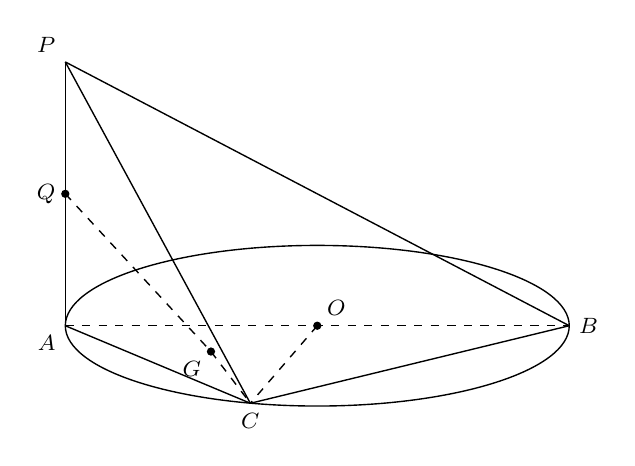
\begin{tikzpicture}[font=\footnotesize, line width=0.5pt, scale=1]
  \coordinate (O) at (0,0);
  \coordinate (A) at (-3.2,0);
  \coordinate (B) at (3.2,0);
  \coordinate (C) at (-0.85,-0.985);
  \coordinate (P) at (-3.2,3.35);
  \coordinate (Q) at (-3.2,1.675);
  \coordinate (G) at (-1.35,-0.328);
  % 底面圆（斜二测画法下的椭圆）
  \draw (0,0) ellipse (3.2 and 1.02);
  % 可见棱
  \draw (P) -- (A);
  \draw (P) -- (B);
  \draw (P) -- (C);
  \draw (A) -- (C);
  \draw (C) -- (B);
  % 被遮挡的线
  \draw[dashed] (A) -- (B);
  \draw[dashed] (O) -- (C);
  \draw[dashed] (Q) -- (G);
  \draw[dashed] (G) -- (C);
  % 点与标签
  \fill (O) circle (1.5pt) node[above right] {$O$};
  \fill (Q) circle (1.5pt) node[left] {$Q$};
  \fill (G) circle (1.5pt) node[below left] {$G$};
  \node[above left] at (P) {$P$};
  \node[below left] at (A) {$A$};
  \node[right] at (B) {$B$};
  \node[below] at (C) {$C$};
\end{tikzpicture}
\end{center}
\nopagebreak[4]
\Needspace{4\baselineskip}
\textbf{解析}
\Needspace{5\baselineskip}
\textbf{（1）} 因为 $AB$ 是圆的直径，$C$ 在圆上，由直径所对的圆周角为直角得
\nopagebreak[4]
\[BC\perp AC.\]
\Needspace{5\baselineskip}
又 $PA\perp$ 圆所在的平面，而 $BC$ 在该平面内，所以
\nopagebreak[4]
\[PA\perp BC.\]
\Needspace{5\baselineskip}
$PA$，$AC$ 是平面 $PAC$ 内两条相交直线，故
\nopagebreak[4]
\[BC\perp\text{\text{平面} }PAC.\]

\Needspace{5\baselineskip}
\textbf{（2）} 取 $AC$ 的中点 $N$，连接 $ON$。在 $\triangle ABC$ 中，$O$ 是 $AB$ 的中点，$N$ 是 $AC$ 的中点，故
\nopagebreak[4]
\[ON\parallel BC.\]
\Needspace{5\baselineskip}
因为 $G$ 是 $\triangle AOC$ 的重心，所以 $G$ 在 $\triangle AOC$ 的中线 $ON$ 上，从而
\nopagebreak[4]
\[OG\parallel BC.\]
\Needspace{5\baselineskip}
在 $\triangle PAB$ 中，$Q$ 是 $PA$ 的中点，$O$ 是 $AB$ 的中点，故中位线
\nopagebreak[4]
\[QO\parallel PB.\]
\Needspace{5\baselineskip}
于是平面 $QOG$ 内两条相交直线 $QO$，$OG$ 分别平行于平面 $PBC$ 内的两条相交直线 $PB$，$BC$，所以
\nopagebreak[4]
\[\text{\text{平面} }QOG\parallel\text{\text{平面} }PBC.\]
\Needspace{5\baselineskip}
又 $QG\subset$ 平面 $QOG$，故
\nopagebreak[4]
\[QG\parallel\text{\text{平面} }PBC.\]

\gkanswer{答案（1）：证明见解析。}

\gkanswer{答案（2）：证明见解析。}

\end{answer}
\begin{answer}
\gksolhead{19}{}

\textbf{题目}：

现有 $6$ 道题，其中 $4$ 道甲类题，$2$ 道乙类题，张同学从中任取 $2$ 道题解答。试求：

（1） 所取的 $2$ 道题都是甲类题的概率；

（2） 所取的 $2$ 道题不是同一类题的概率。

\Needspace{4\baselineskip}
\textbf{解析}
\Needspace{5\baselineskip}
\textbf{（1）} 从 $6$ 道题中任取 $2$ 道，共有 $\mathrm C_6^2=15$ 种等可能取法。所取 $2$ 道都是甲类题，即从 $4$ 道甲类题中取 $2$ 道，有 $\mathrm C_4^2=6$ 种，故所求概率为
\nopagebreak[4]
\[P_1=\frac{\mathrm C_4^2}{\mathrm C_6^2}=\frac6{15}=\frac25.\]

\Needspace{5\baselineskip}
\textbf{（2）} “不是同一类题”即“一道甲类、一道乙类”，取法有 $4\times2=8$ 种，故
\nopagebreak[4]
\[P_2=\frac{4\times2}{\mathrm C_6^2}=\frac8{15}.\]
（也可用对立事件：$1-\dfrac{\mathrm C_4^2+\mathrm C_2^2}{15}=1-\dfrac7{15}=\dfrac8{15}$。）

\gkanswer{答案（1）：$\dfrac25$。}

\gkanswer{答案（2）：$\dfrac8{15}$。}

\end{answer}
\begin{answer}
\gksolhead{20}{}

\textbf{题目}：

如图，抛物线 $C_1:x^2=4y$，$C_2:x^2=-2py\ (p>0)$。点 $M(x_0,y_0)$ 在抛物线 $C_2$ 上，过 $M$ 作 $C_1$ 的切线，切点为 $A$，$B$（$M$ 为原点 $O$ 时，$A$，$B$ 重合于 $O$）。当 $x_0=1-\sqrt2$ 时，切线 $MA$ 的斜率为 $-\dfrac12$。

（1） 求 $p$ 的值；

（2） 当 $M$ 在 $C_2$ 上运动时，求线段 $AB$ 中点 $N$ 的轨迹方程（$A$，$B$ 重合于 $O$ 时，中点为 $O$）。
\nopagebreak[4]
\begin{center}% 2013 辽宁卷文科第 20 题：抛物线 C1、C2 与过 M 的两条切线。
\begin{tikzpicture}[font=\footnotesize, line width=0.5pt, >=Stealth, scale=1.15]
  % 坐标轴
  \draw[->] (-3.3,0) -- (3.5,0) node[below] {$x$};
  \draw[->] (0,-2.8) -- (0,2.9) node[right] {$y$};
  \node[below right] at (0,0) {$O$};
  % C1: x^2=4y, 即 y=x^2/4
  \draw[domain=-3.15:3.15, smooth, samples=120] plot (\x,{\x*\x/4});
  % C2: x^2=-4y, 即 y=-x^2/4
  \draw[domain=-3.15:3.15, smooth, samples=120] plot (\x,{-\x*\x/4});
  % M(-1,-0.25) 在 C2 上；两条切线的切点
  \coordinate (M) at (-1,-0.25);
  \coordinate (A) at (-2.4142,1.4572);
  \coordinate (B) at (0.4142,0.0429);
  \draw ($(M)!-0.25!(A)$) -- ($(M)!1.22!(A)$);
  \draw ($(M)!-0.25!(B)$) -- ($(M)!1.55!(B)$);
  \fill (M) circle (1.4pt) node[below right] {$M$};
  \node[above] at (A) {$A$};
  \node[above right] at (B) {$B$};
\end{tikzpicture}
\end{center}
\nopagebreak[4]
\Needspace{4\baselineskip}
\textbf{解析}
\Needspace{5\baselineskip}
\textbf{（1）} 设切点 $A\left(t,\dfrac{t^2}4\right)$。由 $y=\dfrac{x^2}4$ 得 $y'=\dfrac x2$，故 $C_1$ 在 $A$ 处的切线为
\nopagebreak[4]
\[y=\frac t2x-\frac{t^2}4.\]
\Needspace{5\baselineskip}
它过 $M(x_0,y_0)$，代入得
\nopagebreak[4]
\[t^2-2x_0t+4y_0=0. \tag{①}\]
两条切线的切点对应的参数 $t_1$，$t_2$ 是方程①的两根，且切线斜率分别为 $\dfrac{t_1}2$，$\dfrac{t_2}2$。

\Needspace{5\baselineskip}
已知切线 $MA$ 的斜率为 $-\dfrac12$，故 $t_1=-1$。将 $t=-1$ 代入①：
\nopagebreak[4]
\[1+2x_0+4y_0=0.\]
\Needspace{5\baselineskip}
由 $x_0=1-\sqrt2$ 得
\nopagebreak[4]
\[4y_0=-1-2(1-\sqrt2)=2\sqrt2-3,\qquad y_0=\frac{2\sqrt2-3}4.\]
\Needspace{5\baselineskip}
又 $M$ 在 $C_2:x^2=-2py$ 上，故
\nopagebreak[4]
\[(1-\sqrt2)^2=-2p\cdot\frac{2\sqrt2-3}4.\]
\Needspace{5\baselineskip}
左边 $(1-\sqrt2)^2=3-2\sqrt2$，右边 $=-p\cdot\dfrac{2\sqrt2-3}2=\dfrac{p(3-2\sqrt2)}2$。由 $3-2\sqrt2\neq0$ 得
\nopagebreak[4]
\[\frac p2=1,\qquad p=2.\]

\Needspace{5\baselineskip}
\textbf{（2）} 设 $A$，$B$ 对应的参数为 $t_1$，$t_2$，由①及韦达定理
\nopagebreak[4]
\[t_1+t_2=2x_0,\qquad t_1t_2=4y_0.\]
\Needspace{5\baselineskip}
线段 $AB$ 的中点 $N(x,y)$ 满足
\nopagebreak[4]
\[x=\frac{t_1+t_2}2=x_0,\]
\nopagebreak[4]
\[y=\frac18\left(t_1^2+t_2^2\right)=\frac18\left[(t_1+t_2)^2-2t_1t_2\right]
=\frac{4x_0^2-8y_0}8=\frac{x_0^2-2y_0}2.\]
\Needspace{5\baselineskip}
由（1）知 $p=2$，即 $C_2:x^2=-4y$，故 $y_0=-\dfrac{x_0^2}4$。代入得
\nopagebreak[4]
\[y=\frac{x_0^2+\dfrac{x_0^2}2}2=\frac34x_0^2.\]
\Needspace{5\baselineskip}
又 $x=x_0$，所以
\nopagebreak[4]
\[y=\frac34x^2,\quad\text{\text{即}}\quad x^2=\frac43y.\]

\Needspace{5\baselineskip}
反之，对任意实数 $x_0$，取 $M\left(x_0,-\dfrac{x_0^2}4\right)\in C_2$，方程①的判别式
\nopagebreak[4]
\[\Delta=4x_0^2-16y_0=4x_0^2+4x_0^2=8x_0^2\geqslant0,\]
\Needspace{5\baselineskip}
两条切线（$x_0=0$ 时重合于 $O$）存在，对应中点 $N\left(x_0,\dfrac34x_0^2\right)$。故所求轨迹方程为
\nopagebreak[4]
\[y=\frac34x^2\quad(x\in\mathbf R).\]

\gkanswer{答案（1）：$p=2$。}

\gkanswer{答案（2）：$y=\dfrac34x^2$（即 $x^2=\dfrac43y$，$x\in\mathbf R$）。}

\end{answer}
\begin{answer}
\gksolhead{21}{}

\textbf{题目}：

（1） 证明：当 $x\in[0,1]$ 时，$\dfrac{\sqrt2}2x\leqslant\sin x\leqslant x$；

（2） 若不等式 $ax+x^2+\dfrac{x^3}2+2(x+2)\cos x\leqslant4$ 对 $x\in[0,1]$ 恒成立，求实数 $a$ 的取值范围。

\Needspace{4\baselineskip}
\textbf{解析}
\Needspace{5\baselineskip}
\textbf{（1）} 先证右边。令
\nopagebreak[4]
\[u(x)=x-\sin x,\qquad x\in[0,1].\]
\Needspace{5\baselineskip}
则 $u'(x)=1-\cos x\geqslant0$，$u(x)$ 在 $[0,1]$ 上单调递增，且 $u(0)=0$，故 $u(x)\geqslant0$，即
\nopagebreak[4]
\[\sin x\leqslant x.\]

\Needspace{5\baselineskip}
再证左边。令
\nopagebreak[4]
\[v(x)=\sin x-\frac{\sqrt2}2x,\qquad x\in[0,1].\]
\Needspace{5\baselineskip}
则
\nopagebreak[4]
\[v'(x)=\cos x-\frac{\sqrt2}2.\]
\Needspace{5\baselineskip}
当 $x\in\left[0,\dfrac\pi4\right)$ 时 $v'(x)>0$，当 $x\in\left(\dfrac\pi4,1\right]$ 时 $v'(x)<0$，故 $v$ 在 $\left[0,\dfrac\pi4\right]$ 上递增、在 $\left[\dfrac\pi4,1\right]$ 上递减，最小值在端点处取得。计算
\nopagebreak[4]
\[v(0)=0,\qquad v(1)=\sin1-\frac{\sqrt2}2.\]
\Needspace{5\baselineskip}
因为 $1>\dfrac\pi4$ 且 $\sin x$ 在 $\left[0,\dfrac\pi2\right]$ 上递增，所以 $\sin1>\sin\dfrac\pi4=\dfrac{\sqrt2}2$，即 $v(1)>0$。故 $v(x)\geqslant0$，即
\nopagebreak[4]
\[\frac{\sqrt2}2x\leqslant\sin x.\]
\Needspace{5\baselineskip}
综上，当 $x\in[0,1]$ 时
\nopagebreak[4]
\[\frac{\sqrt2}2x\leqslant\sin x\leqslant x.\]

\Needspace{5\baselineskip}
\textbf{（2）} $x=0$ 时原不等式为 $4\leqslant4$，对任意 $a$ 成立。以下设 $x\in(0,1]$，不等式等价于
\nopagebreak[4]
\[a\leqslant h(x):=\frac{4-x^2-\dfrac{x^3}2-2(x+2)\cos x}{x}.\]
\Needspace{5\baselineskip}
令
\nopagebreak[4]
\[\varphi(x)=4+2x-x^2-\frac{x^3}2-2(x+2)\cos x,\]
则 $h(x)=\dfrac{\varphi(x)}x-2$。下面证明 $\varphi(x)\geqslant0$，从而 $h(x)\geqslant-2$；又当 $x\to0^+$ 时 $\varphi(x)\to0$，故 $h(x)\to\varphi'(0)-2=-2$。

\Needspace{5\baselineskip}
求导：
\nopagebreak[4]
\[\varphi'(x)=2-2x-\frac32x^2-2\cos x+2(x+2)\sin x,\]
\nopagebreak[4]
\[\varphi''(x)=-2-3x+4\sin x+2(x+2)\cos x,\]
\nopagebreak[4]
\[\varphi'''(x)=-3+6\cos x-2(x+2)\sin x,\]
\nopagebreak[4]
\[\varphi''''(x)=-8\sin x-2(x+2)\cos x<0\quad(0<x\leqslant1).\]
\Needspace{5\baselineskip}
所以 $\varphi'''$ 在 $[0,1]$ 上严格递减。又
\nopagebreak[4]
\[\varphi'''(0)=3>0,\qquad \varphi'''(1)=-3+6\cos1-6\sin1\approx-4.81<0,\]
故 $\varphi'''$ 在 $(0,1)$ 内有唯一零点 $x_0$。于是 $\varphi''$ 在 $[0,x_0]$ 上递增、在 $[x_0,1]$ 上递减，最大值在 $x_0$ 处。

\Needspace{5\baselineskip}
而
\nopagebreak[4]
\[\varphi''(0)=2>0,\qquad \varphi''(1)=-5+4\sin1+6\cos1\approx1.61>0,\]
\Needspace{5\baselineskip}
（数值复核：$\sin1\approx0.8415$，$\cos1\approx0.5403$）故 $\varphi''(x)>0$ 在 $[0,1]$ 上恒成立。于是 $\varphi'$ 在 $[0,1]$ 上递增，结合 $\varphi'(0)=0$ 得 $\varphi'(x)\geqslant0$；从而 $\varphi$ 在 $[0,1]$ 上递增，结合 $\varphi(0)=0$ 得
\nopagebreak[4]
\[\varphi(x)\geqslant0,\qquad x\in[0,1].\]
\Needspace{5\baselineskip}
因此 $h(x)=\dfrac{\varphi(x)}x-2\geqslant-2$，且当 $x\to0^+$ 时 $h(x)\to-2$。若 $a> -2$，取充分小的 $x>0$ 可使 $h(x)<a$，原不等式不成立；故必须 $a\leqslant-2$，而 $a=-2$ 时不等式对一切 $x\in[0,1]$ 成立。所以 $a$ 的取值范围是
\nopagebreak[4]
\[a\leqslant-2,\quad\text{\text{即}}\quad a\in(-\infty,-2].\]

\gkanswer{答案（1）：证明见解析。}

\gkanswer{答案（2）：$a\leqslant-2$。}

\end{answer}
\begin{answer}
\gksolhead{22}{}

\textbf{题目}：

如图，$AB$ 为 $\odot O$ 直径，直线 $CD$ 与 $\odot O$ 相切于 $E$，$AD$ 垂直 $CD$ 于 $D$，$BC$ 垂直 $CD$ 于 $C$，$EF$ 垂直 $AB$ 于 $F$，连接 $AE$，$BE$。证明：

（1） $\angle FEB=\angle CEB$；

（2） $EF^2=AD\cdot BC$。
\nopagebreak[4]
\begin{center}% 2013 辽宁卷文科第 22 题：AB 为 ⊙O 直径，CD 切 ⊙O 于 E，AD⊥CD，BC⊥CD，EF⊥AB。
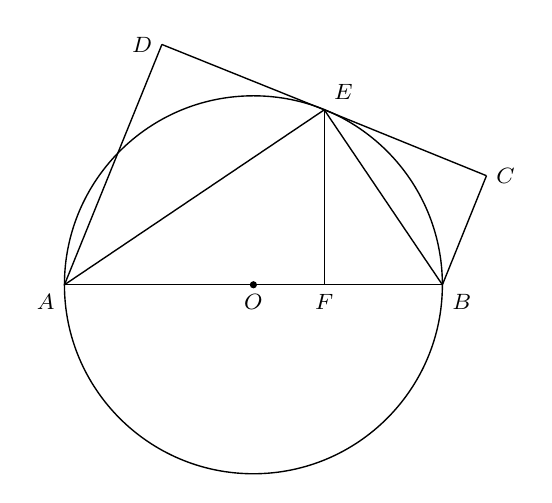
\begin{tikzpicture}[font=\footnotesize, line width=0.5pt, scale=1.0]
  \coordinate (O) at (0,0);
  \coordinate (A) at (-2.4,0);
  \coordinate (B) at (2.4,0);
  \coordinate (E) at (0.90,2.222);
  \coordinate (F) at (0.90,0);
  \coordinate (D) at (-1.162,3.052);
  \coordinate (C) at (2.960,1.385);
  % 圆
  \draw (O) circle (2.4);
  % 直径与切线
  \draw (A) -- (B);
  \draw (D) -- (E) -- (C);
  % 垂线
  \draw (A) -- (D);
  \draw (B) -- (C);
  \draw (E) -- (F);
  % 连接 AE、BE
  \draw (A) -- (E);
  \draw (B) -- (E);
  % 点与标签
  \fill (O) circle (1.3pt) node[below] {$O$};
  \node[below left] at (A) {$A$};
  \node[below right] at (B) {$B$};
  \node[above right] at (E) {$E$};
  \node[left] at (D) {$D$};
  \node[right] at (C) {$C$};
  \node[below] at (F) {$F$};
\end{tikzpicture}
\end{center}
\nopagebreak[4]
\Needspace{4\baselineskip}
\textbf{解析}
\Needspace{5\baselineskip}
\textbf{（1）} 因为 $CD$ 与 $\odot O$ 相切于 $E$，所以
\nopagebreak[4]
\[OE\perp CD.\]
\Needspace{5\baselineskip}
在 $\triangle OEB$ 中 $OE=OB$，故
\nopagebreak[4]
\[\angle OEB=\angle OBE.\]
\Needspace{5\baselineskip}
由 $OE\perp CE$ 得
\nopagebreak[4]
\[\angle CEB=90^\circ-\angle OEB=90^\circ-\angle OBE.\]
\Needspace{5\baselineskip}
又 $EF\perp AB$，在 $\mathrm{Rt}\triangle EFB$ 中
\nopagebreak[4]
\[\angle FEB=90^\circ-\angle EBF=90^\circ-\angle OBE.\]
\Needspace{5\baselineskip}
两式比较得
\nopagebreak[4]
\[\angle FEB=\angle CEB.\]

\textbf{（2）} 设 $\odot O$ 的半径为 $R$，$\angle EOB=\theta$（图中 $0<\theta<\dfrac\pi2$）。

\Needspace{5\baselineskip}
在 $\mathrm{Rt}\triangle OEF$ 中，
\nopagebreak[4]
\[OF=R\cos\theta,\qquad EF=R\sin\theta.\]
\Needspace{5\baselineskip}
因为 $AD\perp CD$，$OE\perp CD$，所以 $AD\parallel OE$。点 $A$ 到直线 $CD$ 的距离等于点 $O$ 到 $CD$ 的距离 $R$ 再加上 $AO$ 在 $OE$ 方向上的投影 $R\cos\theta$，故
\nopagebreak[4]
\[AD=R+R\cos\theta=R(1+\cos\theta).\]
\Needspace{5\baselineskip}
同理，点 $B$ 到 $CD$ 的距离为
\nopagebreak[4]
\[BC=R-R\cos\theta=R(1-\cos\theta).\]
\Needspace{5\baselineskip}
于是
\nopagebreak[4]
\[AD\cdot BC=R^2(1+\cos\theta)(1-\cos\theta)=R^2\left(1-\cos^2\theta\right)=R^2\sin^2\theta=EF^2.\]
\Needspace{5\baselineskip}
即
\nopagebreak[4]
\[EF^2=AD\cdot BC.\]

\gkanswer{答案（1）：证明见解析。}

\gkanswer{答案（2）：证明见解析。}

\end{answer}
\begin{answer}
\gksolhead{23}{}

\textbf{题目}：

在直角坐标系 $xOy$ 中，以 $O$ 为极点，$x$ 轴正半轴为极轴建立极坐标系。圆 $C_1$、直线 $C_2$ 的极坐标方程分别为 $\rho=4\sin\theta$，$\rho\cos\left(\theta-\dfrac\pi4\right)=2\sqrt2$。

（1） 求 $C_1$ 与 $C_2$ 交点的极坐标；

\Needspace{5\baselineskip}
（2） 设 $P$ 为 $C_1$ 的圆心，$Q$ 为 $C_1$ 与 $C_2$ 交点连线的中点，已知直线 $PQ$ 的参数方程为
\nopagebreak[4]
\[\begin{cases}x=t^3+a,\\[2pt] y=\dfrac b2t^3+1,\end{cases}\quad (t\in\mathbf R\ \text{\text{为参数}})\]
求 $a$，$b$ 的值。

\Needspace{4\baselineskip}
\textbf{解析}
\Needspace{5\baselineskip}
\textbf{（1）} 由 $\rho=4\sin\theta$ 得 $\rho^2=4\rho\sin\theta$，即
\nopagebreak[4]
\[C_1:x^2+y^2=4y\quad\Longleftrightarrow\quad x^2+(y-2)^2=4.\]
\Needspace{5\baselineskip}
由 $\rho\cos\left(\theta-\dfrac\pi4\right)=2\sqrt2$ 得
\nopagebreak[4]
\[\frac{\sqrt2}2(\rho\cos\theta+\rho\sin\theta)=2\sqrt2\quad\Longleftrightarrow\quad C_2:x+y=4.\]
\Needspace{5\baselineskip}
联立 $x^2+y^2=4y$ 与 $y=4-x$：
\nopagebreak[4]
\[x^2+(4-x)^2=4(4-x)\implies 2x^2-4x=0\implies x=0\ \text{\text{或}}\ x=2.\]
\Needspace{5\baselineskip}
对应点为 $(0,4)$，$(2,2)$，其极坐标为
\nopagebreak[4]
\[\left(4,\frac\pi2\right),\qquad \left(2\sqrt2,\frac\pi4\right).\]

\Needspace{5\baselineskip}
\textbf{（2）} $C_1$ 的圆心为 $P(0,2)$；两交点 $(0,4)$，$(2,2)$ 连线的中点为
\nopagebreak[4]
\[Q(1,3).\]
\Needspace{5\baselineskip}
直线 $PQ$ 的斜率为 $\dfrac{3-2}{1-0}=1$，方程为
\nopagebreak[4]
\[y=x+2.\]
\Needspace{5\baselineskip}
把参数方程 $x=t^3+a$，$y=\dfrac b2t^3+1$ 代入，得对一切 $t\in\mathbf R$
\nopagebreak[4]
\[\frac b2t^3+1=t^3+a+2,\]
\Needspace{5\baselineskip}
即
\nopagebreak[4]
\[\left(\frac b2-1\right)t^3=a+1.\]
\Needspace{5\baselineskip}
该式对一切 $t$ 成立，故
\nopagebreak[4]
\[\frac b2-1=0,\qquad a+1=0,\]
\Needspace{5\baselineskip}
解得
\nopagebreak[4]
\[a=-1,\qquad b=2.\]

\gkanswer{答案（1）：$(4,\dfrac\pi2)$，$(2\sqrt2,\dfrac\pi4)$。}

\gkanswer{答案（2）：$a=-1$，$b=2$。}

\end{answer}
\begin{answer}
\gksolhead{24}{}

\textbf{题目}：

已知函数 $f(x)=|x-a|$，其中 $a>1$。

（1） 当 $a=2$ 时，求不等式 $f(x)\geqslant4-|x-4|$ 的解集；

（2） 已知关于 $x$ 的不等式 $|f(2x+a)-2f(x)|\leqslant2$ 的解集为 $\{x\mid 1\leqslant x\leqslant2\}$，求 $a$ 的值。

\Needspace{4\baselineskip}
\textbf{解析}
\Needspace{5\baselineskip}
\textbf{（1）} $a=2$ 时 $f(x)=|x-2|$，不等式为
\nopagebreak[4]
\[|x-2|+|x-4|\geqslant4.\]
分段讨论：

\begin{itemize}
\item 当 $x\leqslant2$ 时，$|x-2|+|x-4|=(2-x)+(4-x)=6-2x$，由 $6-2x\geqslant4$ 得 $x\leqslant1$；
\item 当 $2<x<4$ 时，$|x-2|+|x-4|=(x-2)+(4-x)=2<4$，无解；
\item 当 $x\geqslant4$ 时，$|x-2|+|x-4|=(x-2)+(x-4)=2x-6$，由 $2x-6\geqslant4$ 得 $x\geqslant5$。
\end{itemize}

\Needspace{5\baselineskip}
故解集为
\nopagebreak[4]
\[(-\infty,1]\cup[5,+\infty).\]

\Needspace{5\baselineskip}
\textbf{（2）} 因为
\nopagebreak[4]
\[f(2x+a)=|(2x+a)-a|=2|x|,\qquad 2f(x)=2|x-a|,\]
\Needspace{5\baselineskip}
所以原不等式等价于
\nopagebreak[4]
\[\bigl||x|-|x-a|\bigr|\leqslant2,\quad\text{\text{即}}\quad -1\leqslant|x|-|x-a|\leqslant1.\]
\Needspace{5\baselineskip}
记 $g(x)=|x|-|x-a|$。因 $a>1$，分段得
\nopagebreak[4]
\[g(x)=\begin{cases}
-a,&x\leqslant0,\\
2x-a,&0<x<a,\\
a,&x\geqslant a.
\end{cases}\]
\Needspace{5\baselineskip}
故 $|g(x)|\leqslant1$ 等价于
\nopagebreak[4]
\[-1\leqslant2x-a\leqslant1\iff\frac{a-1}2\leqslant x\leqslant\frac{a+1}2.\]
\Needspace{5\baselineskip}
题设解集为 $\{x\mid1\leqslant x\leqslant2\}$，故
\nopagebreak[4]
\[\frac{a-1}2=1,\qquad \frac{a+1}2=2,\]
\Needspace{5\baselineskip}
两式都给出
\nopagebreak[4]
\[a=3.\]

\gkanswer{答案（1）：$(-\infty,1]\cup[5,+\infty)$。}

\gkanswer{答案（2）：$a=3$。}

\end{answer}